The Matlab code used to generate the plots is shown below.
\begin{lstlisting}
% transfer function for robot arm
Plant = tf([1/P.m],[1, P.b/P.m, P.k/P.m]);
C_pid = tf([(P.kd+P.kp*P.sigma),(P.kp+P.ki*P.sigma),P.ki],...
		   [P.sigma,1,0]);
% margin and bode plots 
figure(1), clf, margin(Plant*C_pid), grid on, hold on
bode(Plant*C_pid/(1+Plant*C_pid)) 
legend('Open Loop-Inner', 'Closed Loop-Inner')
\end{lstlisting}
The transfer functions for the plant and controller are defined in Lines~2--3.  The {\tt margin} and {\tt bode} plots of the open and closed loop system respectively, are generated in Lines~6--8.
The results of this code are shown in Figure~\ref{fig:hw_mass_margins}.
\begin{figure}[H]
   \centering
   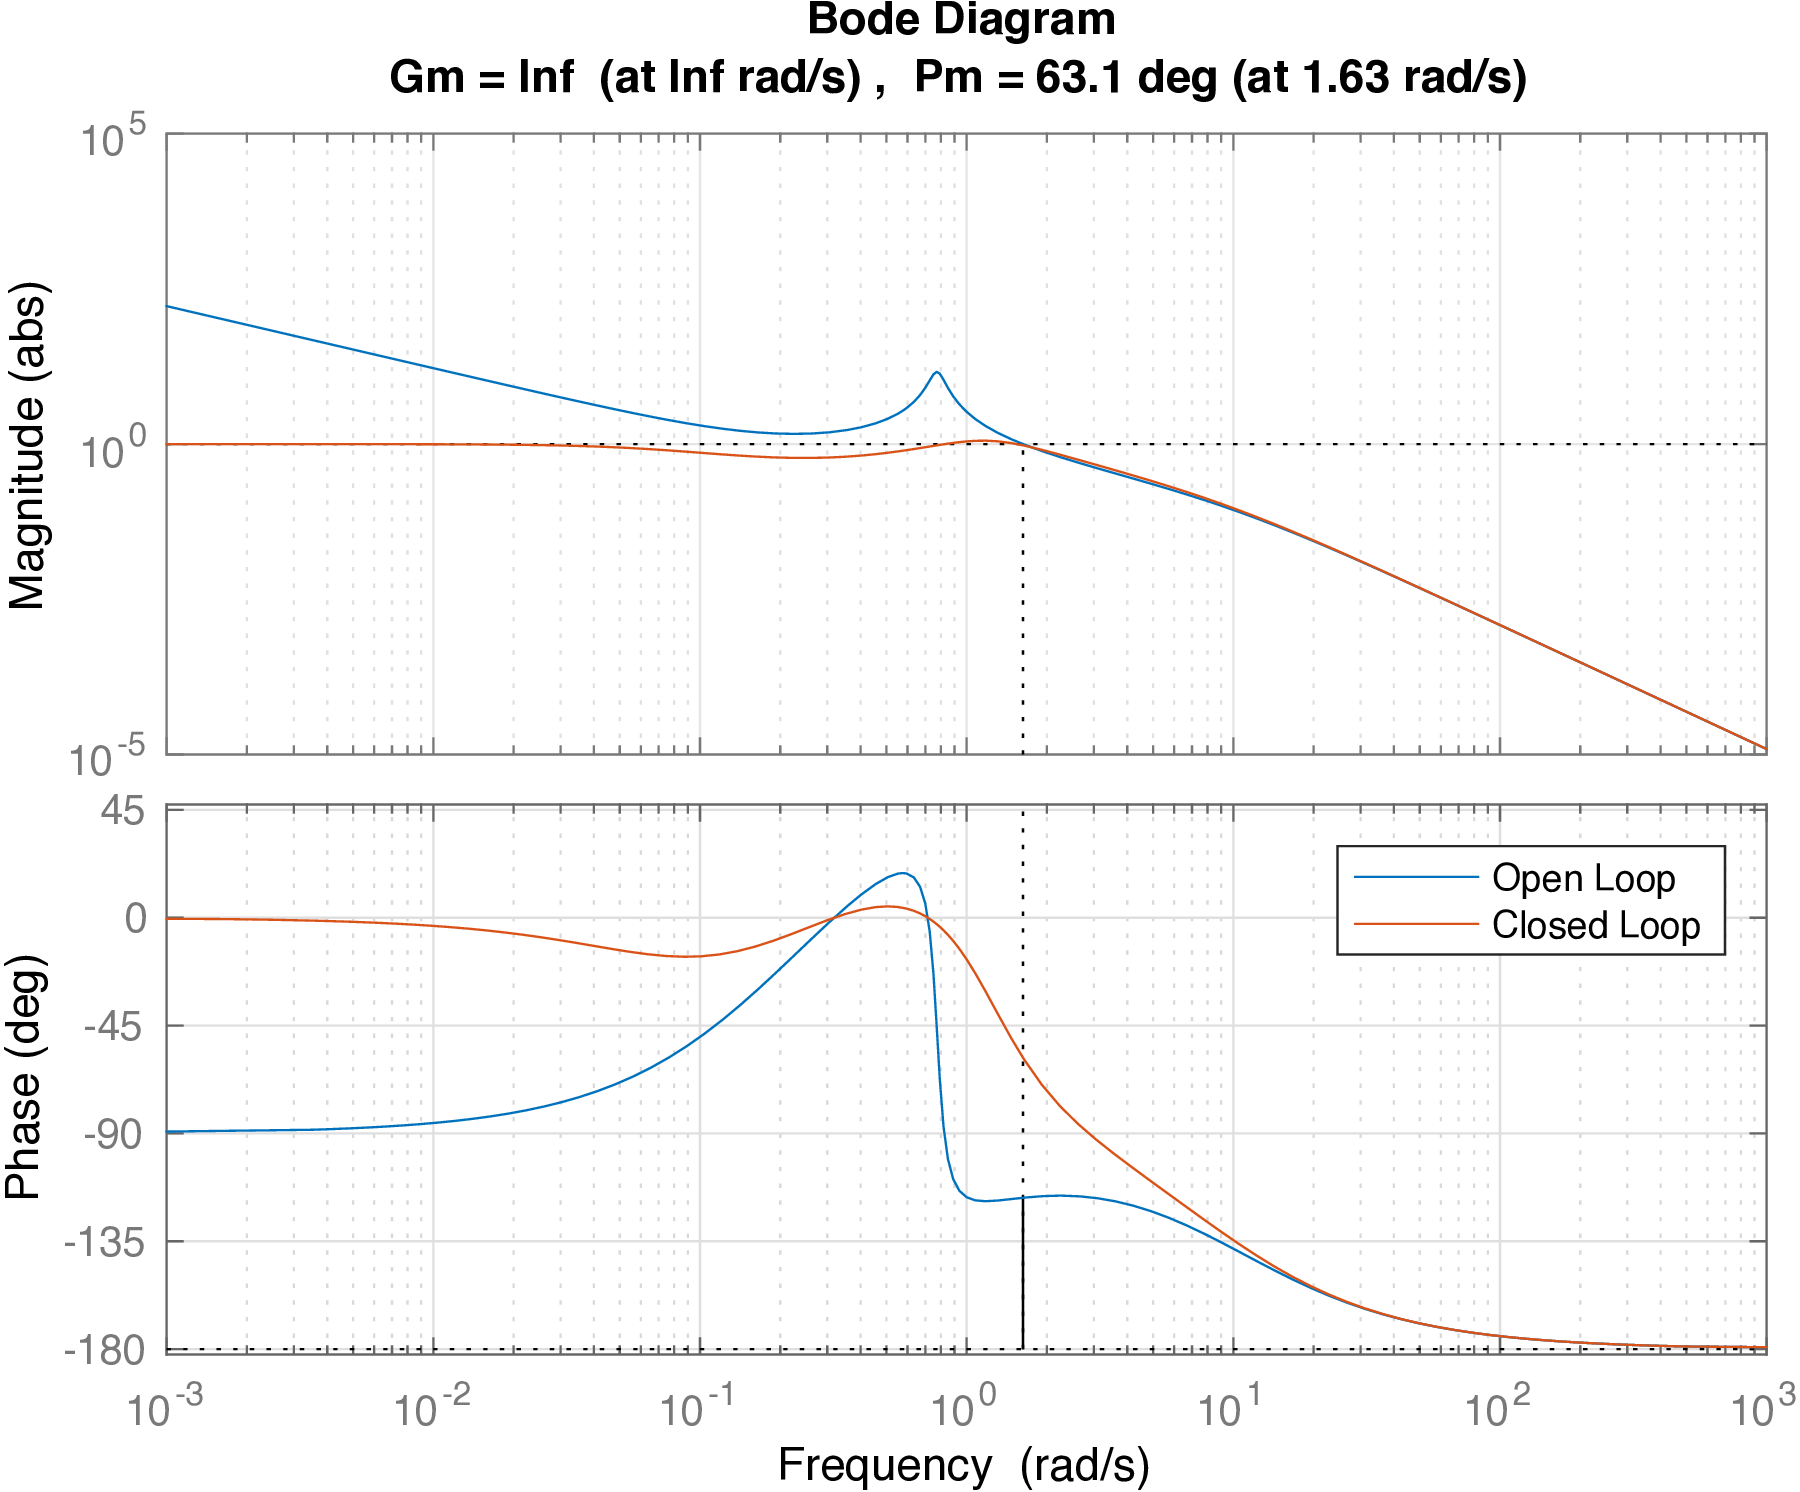
\includegraphics[width=0.95\textwidth]{6_design_studies/figures/hw_mass_margins.pdf}
   \caption{The {\tt margin} plot of the open loop system and the {\tt bode} plot of the closed loop system, of the mass spring damper under PID control.}
   \label{fig:hw_mass_margins}
\end{figure} 

As seen from Figure~\ref{fig:hw_mass_margins} the bandwidth of the closed-loop system is approximately $0.11$~rad/s according to the definition of bandwidth (-3~dB or 0.71 magnitude), which is well below the crossover frequency. This sag in the closed-loop response is due to the low gain in the open-loop system at this frequency and could be remedied by turning up the proportional gain of the PID controller. The second crossing of the -3~dB line occurs at 2.1~rad/s which is in line with expectations for the closed-loop bandwidth given the crossover frequency of the open-loop system that occurs at 1.6~rad/s with a phase margin of 63~deg.
